\singlespacing                        % 设置单倍行距
The research began by establishing three foundational storage methods. 

First, the Ping-pong algorithm, which is a fundamental double-buffering mechanism. When processing a neural network's computation graph, it strictly allocates two independent memory blocks, Buffer A and Buffer B. During inference execution, the current operator reads its input data from Buffer A and writes its computed output into Buffer B. The subsequent operator then reverses these roles, reading from Buffer B and writing to Buffer A. This alternating cycle continues throughout the linear execution, as shown in Figure 2. Although this mechanism extremely simplifies memory management and works efficiently for strictly sequential networks, it inherently struggles with complex topologies involving long skip connections such as residual networks and parallel branches, often resulting in severe memory fragmentation or unfeasible allocations.
\begin{figure}[H]
    \centering
    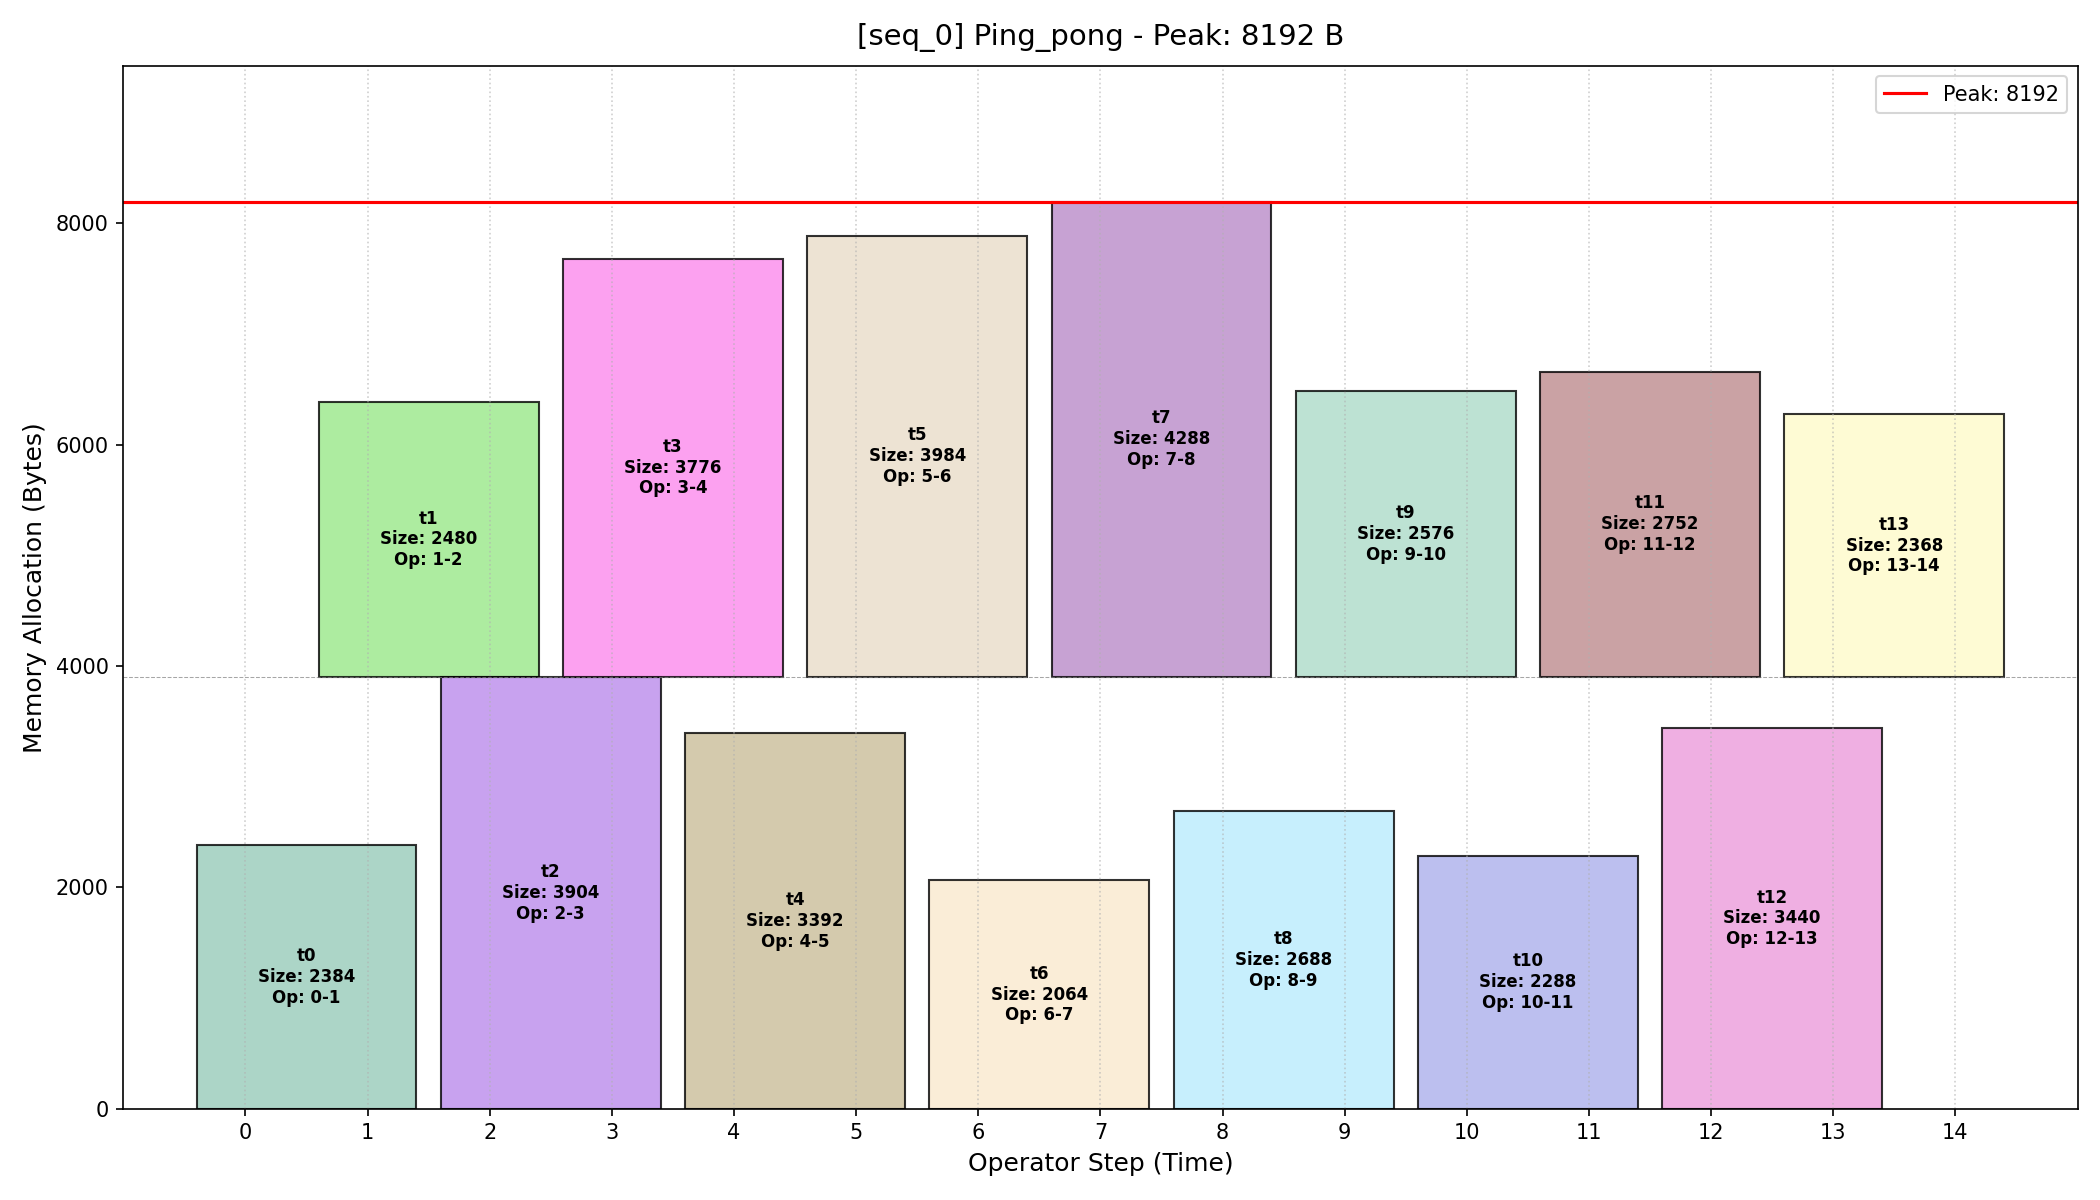
\includegraphics[width = 1\textwidth ]{figures/Memory allocation of Pingpong.png}
    \caption{Memory allocation of Ping-pong algorithm in sequential networks}
    \label{Figure2}
\end{figure}

Secondly, the Greedy by Size algorithm. It employs a discrete bin-packing strategy for memory allocation. The algorithm begins by sorting all tensors in the network in descending order based on their memory footprint, prioritizing the largest tensors first. During the allocation phase, it maintains a dynamic list of discrete shared buffers. For each pending tensor, the algorithm iterates through the existing buffers to check if the tensor's life-cycle temporally overlaps with any tensors already residing in that buffer. If a buffer without temporal conflicts is found, the tensor is assigned to it; if all existing buffers exhibit life-cycle conflicts, an entirely new buffer is created. However, as shown in Figure 3, it suffers from internal fragmentation, as the capacity of each buffer is strictly dictated by its largest resident tensor, leaving unused gaps when smaller tensors occupy the same buffer.
\begin{figure}[H]
    \centering
    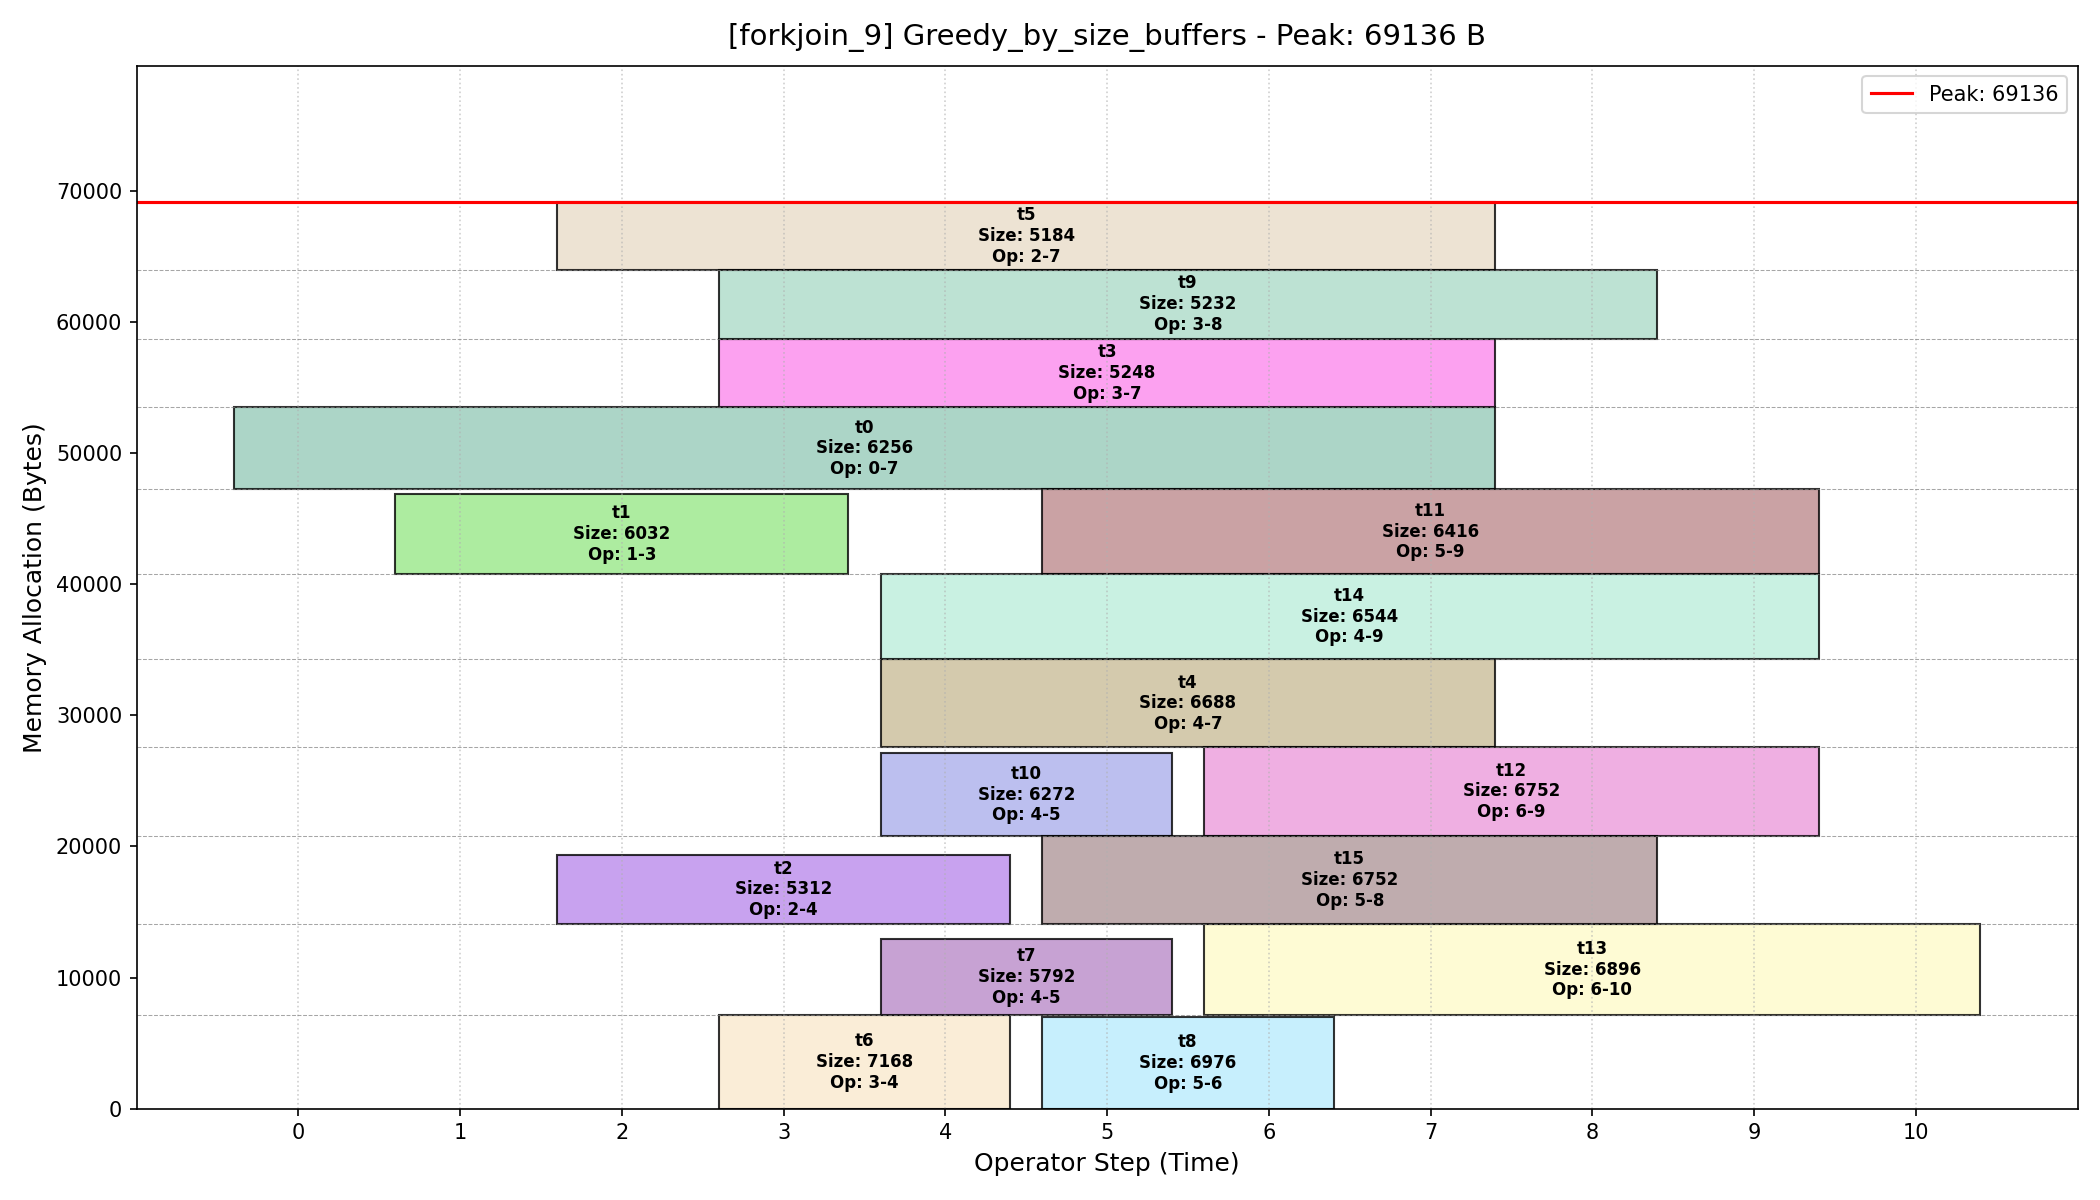
\includegraphics[width = 1\textwidth ]{figures/Memory allocation of Greedy by size buffers.png}
    \caption{Memory allocation of Greedy by Size algorithm in forkjoin networks}
    \label{Figure3}
\end{figure}

Thirdly, the Hole-aware Greedy algorithm, which utilizes an advanced continuous memory placement strategy. Unlike the discrete buffers approach, it treats the entire physical memory as a single, continuous address space (offset). Processing tensors in descending order of size, the algorithm dynamically identifies all previously allocated tensors whose life-cycles temporally overlap with the current tensor. Then it sorted these overlapping tensors by their physical memory offsets. Subsequently, the algorithm precisely measures the spatial gaps between adjacent tensors and employs a "Best-fit" strategy to locate the smallest continuous hole capable of accommodating the new tensor. If no such hole exists, the tensor is placed at the current peak memory boundary. By packing tensors like playing the Tetris game, this strategy aggressively minimizes memory fragmentation and achieves a significantly higher theoretical spatial utilization rate.
\begin{figure}[H]
    \centering
    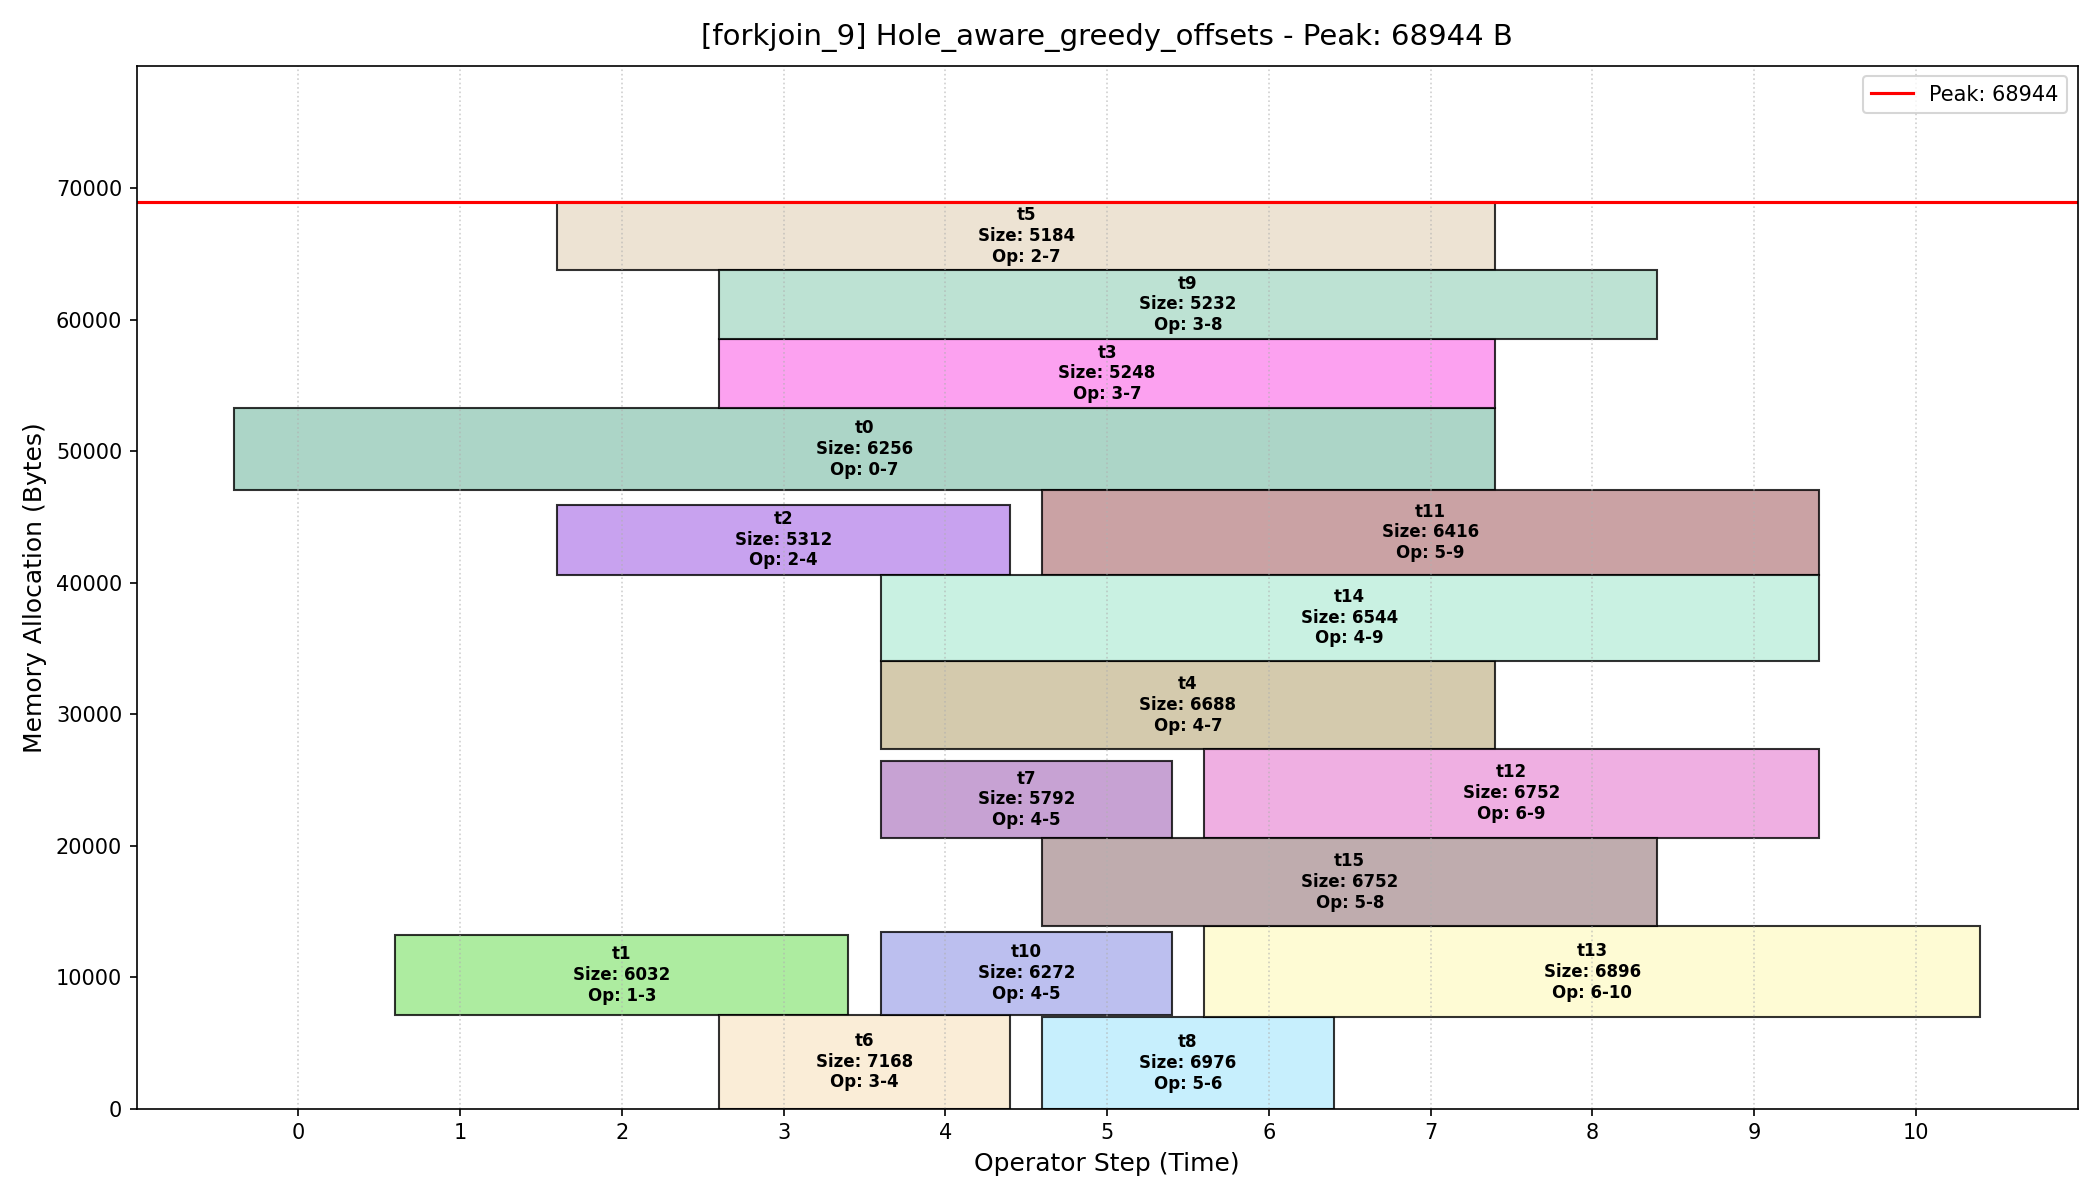
\includegraphics[width = 1\textwidth ]{figures/Memory allocation of Hole aware Greedy.png}
    \caption{Memory allocation of Hole-aware Greedy algorithm in forkjoin networks}
    \label{Figure4}
\end{figure}

By comparing Figure 3 and Figure 4, it is evident that when processing the same task, the Hole-aware Greedy algorithm can achieve a memory allocation strategy with a lower peak memory than the Greedy by Size algorithm.